\documentclass[conference]{IEEEtran}
\IEEEoverridecommandlockouts
\usepackage{amsmath,amssymb,amsfonts}
\usepackage{graphicx}
\usepackage{textcomp}
\usepackage{array}
\usepackage{booktabs}
\usepackage{url}

\begin{document}

\title{Risk-Calibrated Service-Region Routing with Certified Lazy Motion Evaluation for Cleaning Robots}

\author{
\IEEEauthorblockN{Rong Huang and Tingyu Liang\textsuperscript{*}}
\IEEEauthorblockA{Chongqing University of Posts and Telecommunications\\
Chongqing 400065, China\\
Email: 2028701576@qq.com, 2650099818@qq.com}
\thanks{* Corresponding author: Tingyu Liang. Tel: +86 153 1034 6517 (R. Huang), +86 189 2930 7549 (T. Liang).}
}

\maketitle

\begin{abstract}
Cleaning robots often have several feasible base poses for the same target. Reach, approach direction, localization error and clearance decide which poses can be used, and the robot must also choose the visit order. When every transition cost requires a collision-aware motion-planning query, building the full cost matrix can dominate planning. We formulate the task as risk-calibrated service-region routing over finite pose groups. A pose enters a target group only when a one-sided Clopper-Pearson lower confidence bound exceeds the required success probability. Routing uses a mixed graph with admissible bounds for unevaluated directed edges and oracle costs for evaluated edges. The mixed-graph optimum gives a lower bound, and a fully evaluated route gives an upper bound, so the solver reports an anytime certificate relative to the oracle's cost table. A forced-edge bound safely removes directed edges that cannot improve the incumbent. On 135 proxy instances and 24 state-lattice instances, exact queries fell by 57.64 and 59.16 percent while the objective matched the full matrix. An 18-instance continuous-curvature suite and 12 workspaces from real street-network occupancy grids gave query reductions of 36.43 and 48.53 percent. Screening removed another 13.26 and 23.21 percent of queries on these two suites.
\end{abstract}

\begin{IEEEkeywords}
service-region routing, risk calibration, lazy evaluation, optimality certificate, cleaning robots
\end{IEEEkeywords}

\section{Introduction}

A cleaning robot that services a spill, a surface patch or a waste item rarely has one natural base pose. Tool reach and approach direction restrict the usable poses, and localization error and execution error blur the boundary of that set. Fixing one waypoint per target discards useful freedom. Accepting every pose inside a geometric envelope keeps poses whose execution success is often too low.

Pose choice interacts with sequencing. The robot selects one pose from each target group, orders the targets and connects the chosen poses with collision-free motions. Turning, reverse motion and arrival heading make many transitions directed, and some transitions are infeasible. A matrix built from Euclidean distance is cheap but can select a poor route. A matrix built with a motion planner is reliable but expensive, and computing every directed transition can take most of the planning time.

Regional routing, grouped traveling-salesperson formulations and robotic task sequencing are established \cite{isaacs2013,ishida2019,nedjati2020,suare2020}, and multi-goal search with edge bounds and safe pruning is also well studied \cite{chandak2024}. These lines of work do not provide a certified interval on the finite-candidate optimum while the directed cost matrix is still incomplete. This paper addresses the gap. We define service regions from calibrated pose groups, give an exact grouped dynamic program as the reference solver, and develop a lazy procedure that evaluates oracle costs only along optimistic routes while keeping a lower bound from a mixed graph and an upper bound from a fully evaluated route. We also derive a forced-edge bound that removes a directed edge when every route containing it is no better than the incumbent. The certificate covers the finite candidate problem and the oracle's cost table. The continuous service region, the physical motion optimum and the calibration model remain outside it.

\section{Related Work}

The traveling-salesperson problem with neighborhoods replaces point targets with regions, and sampled Dubins configurations turn regional visitation into a generalized traveling-salesperson problem \cite{isaacs2013}. Circular neighborhoods admit nonlinear and two-stage procedures \cite{nedjati2020}, while regional A* plans through a fixed sequence of convex regions \cite{ishida2019}. These formulations treat neighborhoods as deterministic geometry, while our groups follow a statistical acceptance rule. RoboTSP separates task ordering from configuration selection and collision-aware planning \cite{suare2020}, but its proxy does not keep a global interval under oracle costs. IST* uses informed sampling, Steiner-tree updates and safe pruning for fixed terminals \cite{chandak2024}. Our problem has pose groups and directed costs, so the screening condition follows from grouped dynamic programming. Application studies couple grid planning with ordering but build the full matrix first \cite{xiang2022,yang2024,yin2024}. For risk, the Clopper-Pearson bound gives a finite-sample statement for a fixed candidate \cite{clopper1934}, and Bonferroni allocation extends it to a family.

\section{Problem Formulation}

Let $I=\{1,\ldots,m\}$ be the target set. Target $i$ has a finite group of service poses
\begin{equation}
G_i=\{s_i^1,\ldots,s_i^{K_i}\}, \qquad s_i^k=(x_i^k,y_i^k,\theta_i^k)\in SE(2).
\end{equation}
A route selects one pose from each group and visits every group once. For a permutation $\pi$ and selected indices $q_i$, its cost is
\begin{equation}
J(\pi,q)=c(s_0,s_{\pi_1}^{q_{\pi_1}})+\sum_{t=1}^{m-1} c\!\left(s_{\pi_t}^{q_{\pi_t}},s_{\pi_{t+1}}^{q_{\pi_{t+1}}}\right),
\end{equation}
where $s_0$ is the start pose and $c_e\in[0,+\infty]$ is the directed cost of edge $e$. The finite-candidate optimum is $J^\ast=\min_{\pi,q}J(\pi,q)$.

The cost $c_e$ comes from a deterministic oracle and is exact only with respect to that oracle's cost table. In the Hybrid A* oracle, states are merged on a 0.20 m grid with 24 heading bins, and each query is capped at 50,000 expansions. A query that reaches the cap returns $+\infty$. In the 18-instance suite, none of the 463 failed queries reached the cap. A failed query is treated as an infinite edge cost and is not a proof of physical infeasibility. The certificate in this paper is therefore relative to the oracle table, not to the continuous motion optimum.

Each edge also carries a cheap lower bound $\ell_e$ with $0\le \ell_e\le c_e$. Euclidean distance is admissible when oracle costs add non-negative turning, reverse-motion or obstacle terms. The planning objective is to return a feasible route together with an interval
\begin{equation}
LB\le J^\ast\le UB,
\end{equation}
while querying as few oracle edges as possible. At zero requested tolerance the procedure continues until the relative width of the interval is zero within a stated numerical guard.

\section{Method}

\subsection{Risk-Calibrated Pose Groups}

For a fixed pose $s$, a service trial succeeds when the perturbed target and base pose satisfy the reach, heading and clearance tests. With $k_s$ successes in $n_s$ independent trials, the one-sided Clopper-Pearson lower bound is
\begin{equation}
L_s=\mathrm{Beta}^{-1}(\delta_s;k_s,n_s-k_s+1),
\end{equation}
with $L_s=0$ when $k_s=0$. The pose is retained when $L_s\ge 1-\epsilon$, where $\epsilon$ is the allowed per-candidate failure probability. Candidate-wise calibration uses $\delta_s=\delta$. For a family of $K$ candidates, the Bonferroni version uses $\delta_s=\delta/K$, which bounds the probability that any reported bound in the family fails to cover its candidate probability.

\subsection{Grouped Routing and the Certificate}

Subset dynamic programming solves the finite problem exactly. A state $(S,i,k)$ records the lowest cost of a route that has visited the groups in $S$ and ends at $s_i^k$. The recurrence extends the state by one unvisited group and one candidate. With $K=\max_i K_i$, time is $O(2^m m^2 K^2)$ and memory is $O(2^m mK)$. A branch-and-bound backend can replace it without changing the bound logic.

Let $E_q$ be the evaluated edge set. The mixed weight of edge $e$ is
\begin{equation}
w_e(E_q)=
\begin{cases}
c_e, & e\in E_q,\\
\ell_e, & e\notin E_q.
\end{cases}
\end{equation}
Let $LB(E_q)$ be the grouped-route optimum under these weights. Every mixed route cost is no larger than its oracle cost, so minimization over the same route set gives $LB(E_q)\le J^\ast$. Any feasible route whose edges all lie in $E_q$ has cost $UB$, and $J^\ast\le UB$. The solver stops when $UB-LB\le \eta UB+\tau$ with $0\le \eta<1$ and $\tau=10^{-10}$. The returned route then satisfies
\begin{equation}
0\le \frac{UB-J^\ast}{UB}\le \eta+\frac{\tau}{UB}
\end{equation}
when $UB>0$. The division by $UB$ is a convention, because $UB$ is known and positive while $J^\ast$ is not. If $UB=0$ then $J^\ast=0$ and the procedure reports the absolute gap. The guard $\tau$ is part of the stated certificate rather than an implementation detail. We omit longer proofs for space, and the arguments follow directly from the two inequalities.

\subsection{Lazy Evaluation}

The procedure starts with every edge at its lower bound and solves the grouped route on this optimistic graph. It evaluates every edge of the first route and uses the oracle cost as the initial upper bound when the route is feasible. It then alternates between solving the mixed graph, updating the lower bound, and querying one unevaluated edge on the current relaxed route. The edge with the largest lower bound is queried first. This order is a heuristic. Interval validity follows from admissibility and full-route evaluation, not from the order.

For a finite edge set, a deterministic oracle and at least one feasible route, zero-gap execution terminates after finitely many evaluations. Each non-terminal iteration either evaluates a new edge or lowers the upper bound once, and in the latter case the next iteration meets the stopping test. The procedure therefore needs at most $|E|+2$ iterations.

\subsection{Safe Edge Screening}

Lazy evaluation still revisits edges that later prove unable to improve the incumbent. For a directed edge $e$, define
\begin{equation}
LB_e=\min_{r:\,e\in r}\ \sum_{a\in r} w_a,
\end{equation}
which is the best mixed-cost route constrained to contain $e$. Every oracle route containing $e$ costs at least $LB_e$. When $LB_e\ge UB$ and $e$ is unevaluated, removing $e$ preserves the incumbent and the interval.

The bound is computed with a forward table $F$ and a suffix table $T$. For a prefix set $S$, a candidate index $k$ of group $i\in S$, and $j\notin S$,
\begin{equation}
F(S\cup\{j\},j,h)=\min_{i\in S}\min_{k}\left[F(S,i,k)+w(s_i^k,s_j^h)\right],
\end{equation}
with $F(\{i\},i,k)=w(s_0,s_i^k)$. For a remaining set $U$ and $j\in U$,
\begin{equation}
T(U\cup\{j\},i,k)=\min_{j\in U}\min_{h}\left[w(s_i^k,s_j^h)+T(U,j,h)\right],
\end{equation}
with $T(\varnothing,i,k)=0$. For a start edge $e=(s_0,s_j^h)$ the prefix set is empty, so $LB_e=w(s_0,s_j^h)+T(I\setminus\{j\},j,h)$. For a cross edge $e=(s_i^k,s_j^h)$ with $i\neq j$,
\begin{equation}
\begin{split}
LB_e=\min_{S\subseteq I:\,i\in S,\,j\notin S}\big[&F(S,i,k)+w(s_i^k,s_j^h)\\
&+T(I\setminus(S\cup\{j\}),j,h)\big].
\end{split}
\end{equation}
Infinite costs use extended arithmetic, with $x+\infty=\infty$ and an empty minimum equal to $\infty$. The two tables meet at the screened edge, and the construction supports asymmetric costs and one-of-many group selection.

The safety argument is short. The incumbent uses only evaluated edges, so it does not contain $e$. Every route that contains $e$ costs at least $UB$ and cannot improve on the incumbent. An optimal route either has cost equal to $UB$, in which case the incumbent itself is optimal and avoids $e$, or has cost below $UB$, in which case it avoids $e$. In both cases a route attaining $J^\ast$ survives the removal, so the mixed optimum over the remaining routes is still at most $J^\ast$. The implementation applies the test with the same $10^{-10}$ guard, which relaxes the guarantee by that additive amount.

\section{Experiments}

\subsection{Setup}

The proxy oracle adds non-negative turning, direction and obstacle terms to Euclidean distance, with 135 instances over 4 to 6 targets, 2 to 4 candidates, three obstacle densities and five seeds. The lattice oracle runs discrete SE(2) A* on 24 instances.

The Hybrid A* oracle uses continuous states, curved primitives, a 0.20 m duplicate grid and 24 heading bins, with a 50,000-expansion cap. Its 18-instance suite covers shelf aisles, partition rooms and a pillar field, with 4 or 5 targets and three seeds.

Calibration used $\epsilon=0.15$ and 95 percent confidence. In the Hybrid A* suite each candidate received 220 calibration trials under target noise of 0.05 to 0.09 m, base-position noise of 0.04 m, heading noise of 2 degrees, reach limits of 0.45 to 1.05 m, a heading tolerance of 18 degrees, and a clearance test based on the 0.10 m footprint. The calibration sweep used 240 trials and 2500 holdout trials per candidate, 56 candidates per family, and four target uncertainty levels. The confidence family contains all 56 candidates generated before any selection.

The real-map suite crops 12 workspaces from three street-network occupancy grids released with the Moving AI benchmark \cite{sturtevant2012}. Each workspace is 30 or 40 cells at 0.20 m per cell, which gives 6 m and 8 m fields, and uses four or five targets with two seeds. The crop for a given map and scale is fixed, so the seeds change target placement and calibration draws rather than map geometry. The footprint, candidate construction and calibration protocol match the synthetic suites.

We compare the full matrix, a one-shot route that optimizes once on lower bounds and evaluates only that route, the lazy solver, the screened solver, and an adapted IST*-style baseline. The baseline replaces the grouped suffix bound with a minimum-spanning-tree bound and is safe but weaker.

\subsection{Results}

All planned instances were valid. The lazy solver matched the full-matrix objective on every instance. Across the proxy, lattice, Hybrid A* and real-map suites, query reductions were 57.64, 59.16, 36.43 and 48.53 percent, and expansion reductions were 72.38, 34.12 and 51.82 percent. The largest objective difference is $3.6\times10^{-15}$, which is an implementation check and not the certificate itself.

On the Hybrid A* suite, lazy evaluation reduced exact queries by 36.43 percent (95 percent interval 31.0 to 41.8). Screening removed another 13.26 percent (9.6 to 17.1), and expanded states fell by 45.34 percent. The real-map suite gave 48.53 percent (41.5 to 55.3), screening added 23.21 percent (17.7 to 28.5), and expanded states fell by 63.41 percent. Fig.~\ref{fig:results}b gives the per-city breakdown.

\begin{figure}[t]
\centering
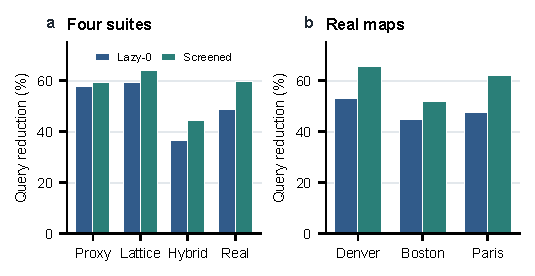
\includegraphics[width=0.92\columnwidth]{figures/fig_results.pdf}
\caption{Exact-query reduction for the four suites (a) and the three real maps (b), with and without safe screening.}
\label{fig:results}
\end{figure}

The one-shot route shows why query savings alone are a poor metric. It used about four exact queries on average but returned an infeasible route in 9 of 18 Hybrid A* instances and 8 of 12 real-map instances. Among the real-map instances where it remained feasible, its objective exceeded the reference by 27.13 percent on average and by 66.78 percent at most. The adapted baseline used 98.9 queries against 99.0 for the lazy solver and 86.2 for the screened solver. It pruned 52.9 edges against 71.3.

\subsection{When Screening Pays}

Screening is not free. On the 24 proxy instances it reduced queries by 0.81 percent and increased runtime by 6.62 times. On the 12 lattice instances the values were 3.91 percent and 1.55 times. On the Hybrid A* suite it removed 13.26 percent of queries and lowered mean runtime to 0.81 times the lazy solver. On the real-map suite the values were 23.21 percent and 0.78, with 11 of 12 instances running faster.

The pattern depends on oracle cost and on how many edges can be pruned. Pillar fields contain long detours whose conditional bound exceeds the incumbent, so screening pays. Shelf aisles contain many infeasible transitions that cannot be pruned early, so the added dynamic programming consumes most of the saving.

Timing was repeated three times on four representative real-map instances with no other work on the machine. Median solve times were 34.12 s for the full matrix, 12.40 s for the lazy solver and 9.06 s for the screened solver. The median lazy-to-full ratio was 0.40 and the screened-to-lazy ratio was 0.72.

\subsection{Risk Calibration}

The sweep reports holdout counts on 896 candidates as sample observations, not ground truth. Fig.~\ref{fig:risk} lists them. Geometric acceptance kept every candidate and 595 fell below the 0.85 threshold on the holdout sample, which gives an observed rate of 66.4 percent with a 95 percent Wilson interval of 63.2 to 69.4 percent. The candidate-wise rule kept 223 candidates and the family-wise rule kept 180, and neither had a holdout failure. With 223 and 180 retained candidates, the one-sided 97.5 percent Clopper-Pearson upper bound on the failure rate is 1.6 percent and 2.0 percent. A zero count is therefore not evidence of zero risk. The family-wise rule kept 43 fewer candidates than the candidate-wise rule and left 121 holdout-passing candidates unselected.

\begin{figure}[t]
\centering
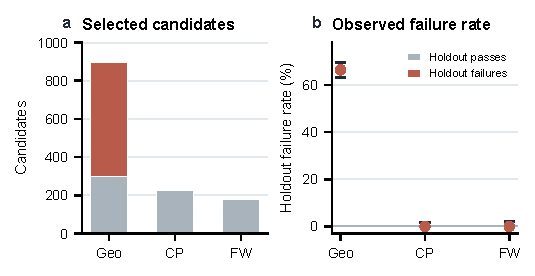
\includegraphics[width=0.92\columnwidth]{figures/fig_risk.pdf}
\caption{Calibration on 896 candidates. (a) Selected candidates split into holdout passes and failures. (b) Observed failure rate with 95 percent intervals; the upper bounds for the two zero counts are 1.6 and 2.0 percent.}
\label{fig:risk}
\end{figure}

\section{Discussion}

The certificate held on 189 instances across four suites. The objective matched the full matrix in every instance, with a largest difference of $3.6\times10^{-15}$, while the certificate is stated up to the $10^{-10}$ guard. Once pose groups and admissible bounds are fixed, lazy evaluation can recover the finite-candidate optimum for a deterministic oracle while querying fewer directed edges. The risk layer changes which poses enter the problem, and the sweep quantifies that cost.

The real-map suite extends the evidence to street-network grids, but these are 6 m and 8 m crops at one resolution and one footprint. They support geometric transfer, not deployment readiness. The disturbances are synthetic, so perception bias, correlated failures and controller drift remain untested. The Hybrid A* implementation is a research prototype with state merging, and the grouped program grows exponentially with the number of targets.

Screening has a clear cost boundary. It pays when one oracle query costs much more than the added dynamic programming and when many edges can be pruned. It does not pay for cheap proxy or lattice oracles. The tree baseline confirms that the value comes from the grouped bound rather than from pruning in general.

\section{Conclusion}

This paper formulates cleaning-task routing as risk-calibrated selection from service-pose groups with expensive directed motion costs. Candidate acceptance uses finite-sample confidence bounds, and routing maintains a certified interval relative to a deterministic oracle while costs are queried on demand. Across four suites the lazy solver matched the reference optimum and reduced exact queries by 36 to 59 percent, and the real-map suite gave 48.53 percent. Safe screening is valid for the grouped directed problem and pays when exact planning is expensive. The next step is a physical cleaning study and site-specific maps. \textbf{Reproducibility.} Code, data and supplementary material are available at \url{https://github.com/Expo-L/self_drive_ai}.

\begin{thebibliography}{00}
\bibitem{isaacs2013} J. T. Isaacs and J. P. Hespanha, ``Dubins traveling salesman problem with neighborhoods: A graph-based approach,'' \emph{Algorithms}, vol. 6, no. 1, pp. 84--99, 2013.
\bibitem{ishida2019} S. Ishida, M. Rigter, and N. Hawes, ``Robot path planning for multiple target regions,'' in \emph{Proc. Eur. Conf. Mobile Robots}, 2019, pp. 1--6.
\bibitem{nedjati2020} A. Nedjati and B. Vizvari, ``Robot path planning by traveling salesman problem with circle neighborhood: Modeling, algorithm, and applications,'' \emph{Comput. Res. Prog. Appl. Sci. Eng.}, vol. 6, no. 4, pp. 288--293, 2020.
\bibitem{suare2020} F. Suarez-Ruiz, T. S. Lembono, and Q.-C. Pham, ``RoboTSP: A fast solution to the robotic task sequencing problem,'' in \emph{Proc. IEEE Int. Conf. Robot. Autom.}, 2018, pp. 1611--1616.
\bibitem{chandak2024} N. Chandak, K. Chour, S. Rathinam, and R. Ravi, ``Informed Steiner trees: Sampling and pruning for multi-goal path finding in high dimensions,'' \emph{IEEE Trans. Autom. Sci. Eng.}, vol. 21, no. 4, pp. 5048--5061, 2024.
\bibitem{sandakalum2022} T. Sandakalum and M. H. Ang Jr., ``Motion planning for mobile manipulators: A systematic review,'' \emph{Machines}, vol. 10, no. 2, art. 97, 2022.
\bibitem{xiang2022} D. Xiang, H. Lin, J. Ouyang, and D. Huang, ``Combined improved A* and greedy algorithm for path planning of multi-objective mobile robot,'' \emph{Sci. Rep.}, vol. 12, art. 13273, 2022.
\bibitem{yang2024} L. Yang et al., ``Multi-area collision-free path planning and efficient task scheduling optimization for autonomous agricultural robots,'' \emph{Sci. Rep.}, vol. 14, art. 18347, 2024.
\bibitem{yin2024} X. Yin, W. Dong, X. Wang, Y. Yu, and D. Yao, ``Route planning of mobile robot based on improved RRT star and TEB algorithm,'' \emph{Sci. Rep.}, vol. 14, art. 8942, 2024.
\bibitem{clopper1934} C. J. Clopper and E. S. Pearson, ``The use of confidence or fiducial limits illustrated in the case of the binomial,'' \emph{Biometrika}, vol. 26, no. 4, pp. 404--413, 1934.
\bibitem{sturtevant2012} N. R. Sturtevant, ``Benchmarks for grid-based pathfinding,'' \emph{IEEE Trans. Comput. Intell. AI Games}, vol. 4, no. 2, pp. 144--148, 2012.
\end{thebibliography}

\end{document}
